\documentclass[aspectratio=169]{beamer}

%=======================
%       IMPORTS
%=======================

\usepackage{amsmath, amsthm, amssymb}   % Math symbols, environments etc.
\usepackage{mathtools}
\usepackage{fontspec}                   % For Unicode fonts
\usepackage{unicode-math}               % For Unicode math fonts
\usepackage{microtype}                  % Nicer interword spacing
\usepackage{polyglossia}                % Provides locale-specific formatting
\usepackage{csquotes}
\usepackage{svg}                        % For including SVG files
\usepackage{booktabs}                   % Nicer tables
\usepackage{tabularx}                   % Allows for linebreaks in tables

\usepackage[
    backend = biber
]{biblatex}

\addbibresource{quaternionen.bib}

% Set beamer theme
\usetheme{metropolis}
% \beamertemplatenavigationsymbolsempty
\metroset
{
    sectionpage = simple,
    subsectionpage = simple
}

\setbeamertemplate{caption}{\raggedright\insertcaption\par}

\usecolortheme{rose}

\setbeamercolor{quote}{fg=black!80!white, bg=blue!10!white}

\setmathfont{TeX Gyre Pagella Math}
\setmonofont[Scale=0.9]{Fira Mono}

\newfontfamily{\mathroman}{TeX Gyre Pagella}[Scale=MatchUppercase]

% Language Setup
\setdefaultlanguage[spelling=new, babelshorthands=true]{german}

% Set path for graphics
\graphicspath{{./graphics/}}

% hyperref setup
\hypersetup
{
    pdfencoding = auto      % For umlauts in PDF sections
}

%=======================
%    CUSTOM COMMANDS
%=======================
\newcommand{\Ham}{\ensuremath{\mathbb{H}}{ }}
\newcommand{\R}{\ensuremath{\mathbb{R}}{ }}

\DeclarePairedDelimiter\abs{\lvert}{\rvert}

\newtheorem{cor}{Korollar}

%=======================
%  DOCUMENT INFORMATION
%=======================

\title{\textsc{Hamilton}sche Quaternionen}
\subtitle{Proseminar Mathematik}
\author[L.~Richardt]{Leon Richardt}
\date[2020-07-07]{7. Juli 2020}
\institute{Universität Osnabrück}

\begin{document}
    \begin{frame}
        \titlepage
    \end{frame}

    \begin{frame}{Überblick}
        \tableofcontents
    \end{frame}

    \section{Reelle Algebren}
    \begin{frame}
        \begin{block}{Anmerkung}
            In dieser Präsentation stehen kleine griechische Buchstaben stets für reelle Zahlen; lateinische Buchstaben stehen für Elemente der momentan betrachteten Algebra.
        \end{block}
    \end{frame}

    \begin{frame}
        \begin{definition}
            Ein Vektorraum \(V\) über \R mit einer Produktabbildung
            \[
                V \times V \to V, (x, y) \mapsto xy
            \]
            heißt \textbf{Algebra} über \R (oder reelle Algebra), wenn die beiden Distributivgesetze
            \begin{gather*}
                (\alpha x + \beta y) z = \alpha \cdot xz + \beta \cdot yz, \\
                x (\alpha y + \beta z) = \alpha \cdot xy + \beta \cdot xz
            \end{gather*}
            für alle \(\alpha, \beta \in \R\) und \(x, y, z \in V\) erfüllt sind.
        \end{definition}
    \end{frame}

    \begin{frame}
        \begin{definition}
            Ein Element \(x\) einer Algebra \(\mathcal{A}\) heißt \textit{Nullteiler}, falls es ein Element \(0 \neq y \in \mathcal{A}\) mit \(xy = 0\) oder \(yx = 0\) gibt.

            Konsequenterweise heißt eine Algebra \textit{nullteilerfrei}, falls sie keine Nullteiler \(\neq 0\) besitzt.
        \end{definition}
    \end{frame}

    \begin{frame}
        \begin{definition}
            Eine Algebra \(\mathcal{A} = (V, \cdot)\) heißt \dots
            \begin{itemize}
                \item
                    \dots{} \textit{assoziativ}, wenn \(x(yz) = (xy)z\) für alle \(x, y, z \in V\) gilt.
                \item
                    \dots{} \textit{kommutativ}, wenn \(xy = xy\) für alle \(x, y \in V\) gilt.
                \item
                    \dots{} \textit{mit Einselement}, wenn es ein Element \(e \in V\) mit \(ex = xe = x\) für alle \(x \in V\) gibt.

                \item
                    \dots{} \textit{Divisionsalgebra}, falls \(\mathcal{A} \neq 0\) und die Gleichungen
                    \[
                        ax = b \text{ und } ya = b
                    \]
                    für alle \(a, b \in V, \, a \neq 0,\) eindeutig lösbar sind.
            \end{itemize}
        \end{definition}
    \end{frame}

    \begin{frame}
        \begin{lemma}
            Folgende Aussagen über eine endlichdimensionale Algebra \(\mathcal{A}\) sind äquivalent:
            \begin{itemize}
                \item[i)]
                    \(\mathcal{A}\) ist Divisionsalgebra.

                \item[ii)]
                    \(\mathcal{A}\) ist nullteilerfrei.
            \end{itemize}
        \end{lemma}
    \end{frame}

    \begin{frame}
        \begin{proof}
            i) \(\implies\) ii) ist klar.

            ii) \(\implies\) i): \\
            Sei \(a \in \mathcal{A} \setminus \{0\}\).
            Die Abbildung \(\varphi \colon \mathcal{A} \to \mathcal{A},\, x \mapsto ax\) ist ein VR-Endomorphismus.
            Wegen der Nullteilerfreiheit ist \(\text{kern}(\varphi) = \{0\}\), was aufgrund des Kernkriteriums die Injektivität bedeutet.
            Da weiterhin \(\dim(\mathcal{A}) < \infty\), folgt aus der Dimensionsformel die Bijektivität.
            Damit ist jede Gleichung der Form \(ax = b\) eindeutig lösbar.

            Die eindeutige Lösbarkeit von \(ya = b\) ergibt sich durch analoge Betrachtung der Abbildung \(y \mapsto ya\).
        \end{proof}
    \end{frame}

    \begin{frame}
        Liegt ein VR \(V\) mit einer Basis \(e_1, \dots, e_n\) vor, so lässt sich durch die Festlegung der \(n^2\) Basisprodukte
        \[
        e_u e_v,\, 1 \leq u, v \leq n,
        \]
        eine Algebra eindeutig bestimmen.
        Denn sind \(x = \sum_{u=1}^{n} \alpha_u e_u\) und  \(y = \sum_{v=1}^{n} \beta_v e_v\) beliebige Elemente in V, so gilt wegen der Distributivgesetze
        \[
            xy = \sum_{u,v=1}^{n} (\alpha_u \beta_v) e_u e_v
        .\]
        Assoziativität und Kommutativität lassen sich dann einfach anhand der Basisprodukte überprüfen.
    \end{frame}


    \section{Historisches}

    \begin{frame}
        \begin{columns}
        \begin{column}{0.5\textwidth}
            \begin{description}
                \item[1805] Geboren in Dublin

                \item[1827] Berufung zum Professor der Astronomie

                \item[1835] Ritterschlag

                \item[1837--1845] Präsident der Royal Irish Academy

                \item[1843] Erfindung der Quaternionen

                \item[1865] Gestorben in Dunsink
            \end{description}
        \end{column}
        \begin{column}{0.5\textwidth}
            \begin{figure}
                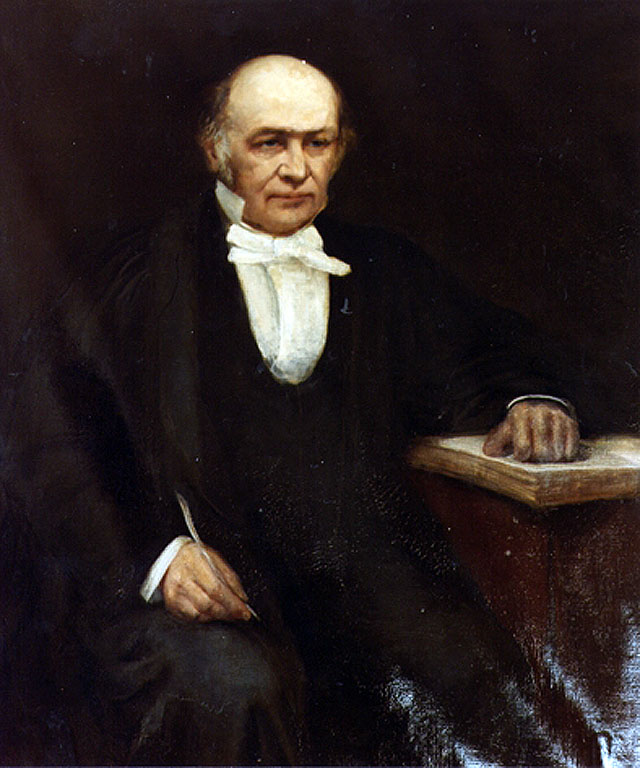
\includegraphics[width=0.8\textwidth]{hamilton_portrait.jpg}
                \caption{Sir William Rowan \textsc{Hamilton} \cite{hamilton_portrait}}
            \end{figure}
        \end{column}
        \end{columns}
    \end{frame}

    \begin{frame}
        \begin{columns}
        \begin{column}{0.5\textwidth}
            \begin{itemize}
                \item
                    Hamilton beschäftigt sich 1835 mit der geometrischen Bedeutung der \emph{komplexen Zahlen} im \(\R^2\)

                \item
                    Er fragt sich:
                    \enquote{Gibt es eine ähnliche Interpretation im \(\R^3\)?}
            \end{itemize}
        \end{column}
        \begin{column}{0.5\textwidth}
            \begin{figure}
                \includesvg[width=\textwidth]{komplexe_multiplikation}
                \caption{Geometrische Interpretation der komplexen Multiplikation \cite{komplexe_multiplikation}}
            \end{figure}
        \end{column}
        \end{columns}
    \end{frame}

    \begin{frame}
    \begin{columns}
    \begin{column}{0.5\textwidth}
        \begin{itemize}
            \item<1->
                Hamilton sucht eine Multiplikation, die die bisherigen Regeln und Beziehungen weiterhin erfüllt.

            \item<2->
                Erster Ansatz: \(x = \alpha + \beta i + \gamma j\) mit \(i^2 = j^2 = -1\).

            \item<3->
                Er stellt fest, dass für die Gültigkeit der Produktregel \(ij + ji = 0\) gelten muss.
                Unter Erhaltung der Kommutativität hieße dies: \(2ij = 0 \implies ij = 0\), was ihm aber nicht gefällt.
        \end{itemize}
    \end{column}
    \begin{column}{0.5\textwidth}
        \begin{beamercolorbox}[wd=\textwidth, rounded=true, shadow=true]{quote}
            \enquote{Well, Papa, can you multiply triplets?}

            \enquote{No, I can only add and subtract them.}

            \vspace{2mm}
            \hfill {\scriptsize--- Gespräch zwischen Hamilton und seinem Sohn}
        \end{beamercolorbox}

        \begin{itemize}
            \item<4->
                Stattdessen gibt Hamilton lieber die Kommutativität auf, was \(ji = -ij \neq 0\) erlaubt.

            \item<5->
                Die entscheidende Idee kommt ihm 1843:\\
                Er setzt \(ij := k, ji = -k\) und nimmt  \(k\) als linear unabhängig von \(i\) und \(j\) an.
        \end{itemize}
        \vfill
    \end{column}
    \end{columns}
    \end{frame}

    \begin{frame}
        \begin{figure}
            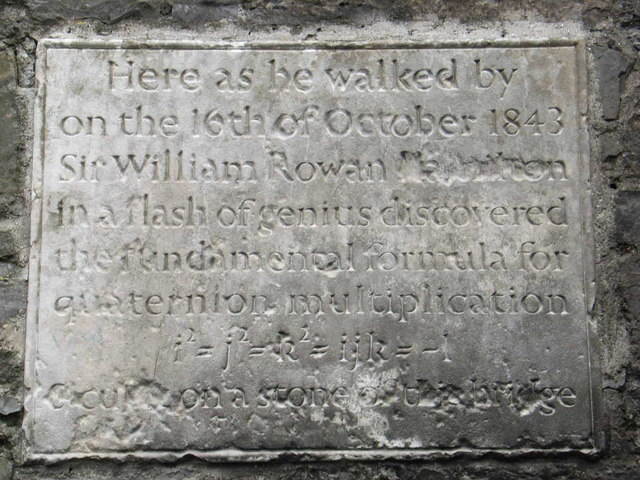
\includegraphics[width=0.7\textwidth]{broome_bridge.jpg}
            \caption{Gedenktafel an der \textit{Broome Bridge} in Dublin \cite{broome_bridge}}
        \end{figure}
    \end{frame}

    \section{Die Quaternionenalgebra \(\mathbb{H}\)}

    \begin{frame}
        Hamilton definiert die \emph{Quaternionen-Algebra} \(\Ham\) durch die Festlegung der Produkte der Basiselemente
        \[
            e_1 := (1,0,0,0), \, e_2 := (0,1,0,0), \, e_3 := (0,0,1,0), \, e_4 := (0,0,0,1):
        \] 
        \centering
        \begin{tabular}{crrr}
                    & \(e_2\) & \(e_3\) & \(e_4\) \\ \midrule
            \(e_2\) & \(- e_1\) & \(e_4\) & \(- e_3\) \\
            \(e_3\) & \(- e_4\) & \(- e_1\) & \(e_2\) \\
            \(e_4\) & \(e_3\) & \(- e_2\) & \(-e _1\)
        \end{tabular}

        \small (Es sei \(e_1\) das Einselement.)

        \raggedright
        \normalsize
        Man sieht direkt, dass \(\Ham\) nicht kommutativ ist.
        Die Assoziativität lässt sich wie im Einführungsabschnitt besprochen überprüfen.
    \end{frame}

    \begin{frame}
        Neben dieser klassischen Konstruktion von \(\Ham\) gibt es noch einen eleganteren Weg, der uns viele Eigenschaften der Quaternionen-Algebra direkter liefert:

        \begin{theorem}
            Die Menge \(\mathcal{H} := \left\{ \begin{pmatrix} w & -z \\ \bar{z} & \bar{w} \end{pmatrix} \colon w, z \in \mathbb{C} \right\}\) ist eine \(\mathbb{R}\)-Unteralgebra von \(\text{\em Mat}(2, \mathbb{C})\) mit Einselement \(E_2\).
            \(\mathcal{H}\) ist eine vierdimensionale, assoziative Divisionsalgebra.
        \end{theorem}
    \end{frame}

    \begin{frame}
        \begin{proof}
            \only<1>{
            Man verifiziert durch Nachrechnen, dass \(\mathcal{H}\) ein vierdimensionaler \(\mathbb{R}\)-UVR von \(\text{Mat}(2, \mathbb{C})\) ist.
            Auch die Abgeschlossenheit bezüglich der Matrizenmultiplikation überprüft man auf diese Weise.

            Die Assoziativität ist klar, da \(\text{Mat}(2, \mathbb{C})\) assoziativ ist.
            }
            \only<2>{
            Um einzusehen, dass \(\mathcal{H}\) auch eine Divisionsalgebra ist, benutzen wir das eingangs bewiesene Nullteilerkriterium:\\
            Seien also \(A, B \in \mathcal{H}\) mit \(AB = 0\).
            Wegen des Determinantenmultiplikationsatzes gilt \(\det(A) \cdot \det(B) = 0\), also \(\det(A) = 0\) oder \(\det(B) = 0\).
            Aus
            \[
                \det \begin{pmatrix} w & -z \\ \bar{z} & \bar{w} \end{pmatrix} = \abs{w}^2 + \abs{z}^2 = 0 \iff w = z = 0
            \]
            folgt
            \[
                AB = 0 \iff A = \begin{pmatrix} 0 & 0 \\ 0 & 0 \end{pmatrix} \text{ oder } B = \begin{pmatrix} 0 & 0 \\ 0 & 0 \end{pmatrix}
            .\] 
            Das bedeutet, dass \(\mathcal{H}\) keine Nullteiler \(\neq 0\) besitzt.
            Damit ist \(\mathcal{H}\) eine Divisionsalgebra.
            }
            \alt<2>{\qedhere}{\phantom\qedhere}
        \end{proof}
    \end{frame}

    \begin{frame}
        \begin{lemma}
            Die Abbildung
            \[
                F \colon \Ham \to \mathcal{H}, \quad (\alpha, \beta, \gamma, \delta) \mapsto
                    \begin{pmatrix}
                        \alpha + \beta i  & - \gamma - \delta i \\
                        \gamma - \delta i & \alpha - \beta i
                    \end{pmatrix}
            ,\]
            ist ein \(\mathbb{R}\)-Algebra-Isomorphismus und es gilt:
            \begin{align*}
                F(e_1) = E_2 =: E,& \quad
                F(e_2) = \begin{pmatrix} i & 0 \\ 0 & -i \end{pmatrix} =: I, \\
                F(e_3) = \begin{pmatrix} 0 & -1 \\ 1 & 0 \end{pmatrix} =: J,& \quad
                F(e_4) = \begin{pmatrix} 0 & -i \\ -i & 0 \end{pmatrix} =: K.
            \end{align*}
        \end{lemma}
    \end{frame}

    \begin{frame}
        \begin{cor}
            Die Hamiltonsche Algebra \Ham ist eine assoziative Divisionsalgebra.
        \end{cor}

        \uncover<2>{
        \begin{proof}
            Wir haben gezeigt, dass \(\mathcal{H}\) eine assoziative Divisionsalgebra ist.

            Durch den oben beschriebenen Isomorphismus \(F\) ist also auch \Ham eine assoziative Divisionsalgebra.
        \end{proof}

        \vfill
        Man muss also \enquote{nur} mit komplexen Matrizen rechnen können, um den Umgang mit der Quaternionen-Algebra zu beherrschen.
        }
    \end{frame}

    \section{Der Imaginärraum von \(\mathbb{H}\)}
    \subsection{Bezug zu klassischen Vektorprodukten}

    \section{Zentrum von \(\mathbb{H}\)}
    \begin{frame}
        \begin{theorem}
            Für die Algebra \Ham gilt:
            \[
                Z \left( \Ham \right) = \R e = \left\{ x \in \Ham \colon xu = ux \,\text{ für alle }\, u \in \Im \left( \Ham \right) \right\}
            .\]
        \end{theorem}
    \end{frame}

    \begin{frame}
        \begin{proof}
            \only<1>{
            Es ist klar, dass \(\R e \subseteq Z \left( \Ham \right) \); denn  \(e\) ist neutrales Element, also per Definition mit allen Elementen aus \(\Ham\) kommutativ.
            Die Skalare sind natürlich ebenfalls kommutativ zueinander.
            }
            \only<2>{
            Zur Umkehrung.\\
            Sei \(x = \alpha e + \beta i + \gamma j + \delta k \in Z \left( \Ham \right)\), das heißt, \(x\) kommutiert mit allen Elementen aus \(\Ham\).
            Insbesondere kommutiert \(x\) mit den Basiselementen \(i, \, j \in \Ham\), es muss also \(ix = xi\) und \(jx = xj\) gelten.

            Wir wollen zeigen, dass dann bereits \(x \in \R e\) ist.
            }
            \only<3>{
            Ausmultiplizieren der ersten Gleichung ergibt
            \begin{alignat*}{3}
                     &&xi &= ix \\
                \iff &&\alpha i - \beta + \gamma k - \delta j &= \alpha i - \beta - \gamma k + \delta j \\
                \iff &&\gamma k - \delta j &= - \gamma k + \delta j \\
                \iff &&\gamma k - \delta j &= - (\gamma k - \delta j) \\
                \iff &&2 \gamma k - 2 \delta j &= 0 \\
                \iff &&\gamma = \delta &= 0.
            \end{alignat*}
            }
            \only<4>{
            Analog ergibt sich aus der zweiten Gleichung \(\beta = \delta = 0\).
            Damit ist \(\beta = \gamma = \delta = 0\).
            \(x\)~ist demnach von der Form \(x = \alpha e\), also \(x \in \R e\).
            Das bedeutet \(Z \left( \Ham \right) \subseteq \R e\), und damit folgt aus dem ersten Teil wie gewünscht
            \[
                Z \left( \Ham \right) = \R e
            .\]
            }
            \alt<4>{\qedhere}{\phantom\qedhere}
        \end{proof}
    \end{frame}

    \section{Endomorphismen von \(\mathbb{H}\)}

    \section{Fundamentalsatz der Algebra für Quaternionen}

    \begin{frame}
        \printbibliography
    \end{frame}
\end{document}
